\section{Methods}
\label{sec:feat_method}

\section{Framework} \label{framework}
Fig. \ref{fig:Framework} illustrates our feature learning and evaluation framework. The individual blocks, such as superpixel segmentation, feature learning methods, and evaluation method, are elaborated in subsequent sections.

\begin{figure}[!htpb]
  \centering
  \includegraphics[width=13cm]{framework/framework}
  \caption[Framework description]{Given a superpixel segmentation and 2D locations, the feature learning algorithm construct a feature matrix $\boldsymbol{X}$, describing each superpixel by a feature. A Random Forest binary classifier is then trained and validated to make predictions of every superpixel. The labels are denoted by $\boldsymbol{y}$, describing if a superpixel belongs to foreground or background. At the bottom-right, we measure the performance of the classifier.}
  \label{fig:Framework}
\end{figure}

Performance evaluation of the different feature learning methods is done on a superpixel level. Hence, the feature learning methods shall output a feature vector for each of the superpixels. Refer to chapter \ref{superpixel_segm} for more details about the superpixel segmentation.

Let $N$ be the number of images in a data sequence and $S$ the number of superpixels over all sequence. As an example, if we have exactly $200$ superpixels per image, we would have $S=N \cdot 200$ superpixels in that sequence. To every superpixel, we want to assign a feature vector of dimension $D$. We can write the sequence feature matrix as $\boldsymbol{X} = [\boldsymbol{x}_1,...,\boldsymbol{x}_S]^T \in \mathbb{R}^{S \times D}$. Let $\boldsymbol{y} = [y_1,...y_S]^T \in \{0,1\}^S$ be the labels, meaning that $y_i=1$ for superpixels that count to the object of interest and $y_i=0$ for superpixels belonging to the background. Using the feature matrix $\boldsymbol{X}$ and the label vector $\boldsymbol{y}$, a random forest classifier then calculates performance measures, such as Precision-Recall curve and \textit{max F1-Score}. How the Random Forest classifier is applied is described in chapter \ref{random_forest}.

Some feature learning methods use the gaze location as an object prior, given as xy-coordinates for each image frame. The green point in Fig. \ref{fig:Framework} illustrates this location.

\section{Superpixel Segmentation} \label{superpixel_segm}
As described above, the performance evaluation is performed on a superpixel level. Having a feature vector for each superpixel instead of each pixel reduces the computational requirements. 

We used the superpixel segmentation algorithm ASLIC proposed in \cite{achanta12}.
The original simple linear iterative clustering (SLIC) relies on k-means clustering performed in color the Lab color space and further uses spatial coordinates of pixels.
A trade-off between color similarity and spatial proximity is necessary.
In the SLIC approach, the problem is solved by using a compactness parameter.
For images with both, flat and very textured regions, using the same compactness parameter lead to smooth regular-sized superpixel in the flat regions and highly irregular sized superpixel in textured regions.
Thus, \cite{a} came up with the ASLIC approach, which adaptively chooses the compactness parameter for each superpixel differently.
Fig. \ref{fig:ExSuperpixel} shows an example of using ASLIC on dataset \textit{Slit-Lamp Retina A}.

\begin{figure}[!htbp]
  \centering
  \label{fig:subfig:example_superpixel}
  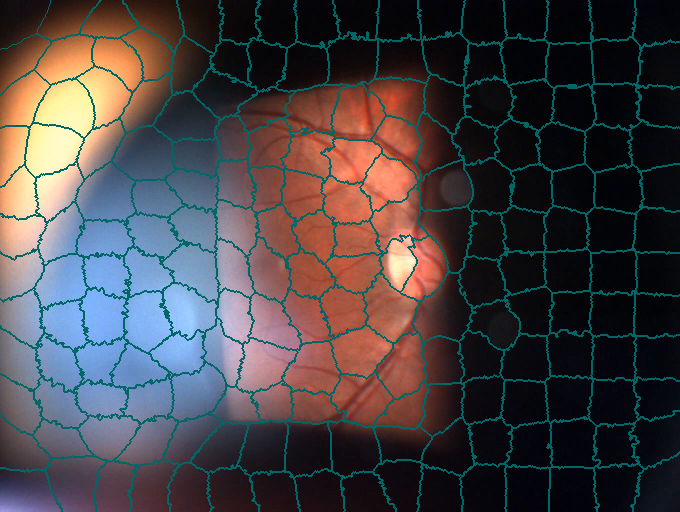
\includegraphics[width=3.5cm]{superpixel_examples/ds12_superpixel}
  \caption[Example of superpixel segmentation]{Example of ASLIC superpixel segmentation on dataset \textit{Slit-Lamp Retina A} with number of superpixels $S=200$. Note the regular shape of superpixels in all regions.}
  \label{fig:ExSuperpixel}
\end{figure}

As parameter, the number of superpixels is crucial. In terms of trade-off, setting a large value will capture the contours of objects more accurately, at the cost of having a higher quantity of samples to predict/classify. We verified that taking $200$ superpixels per frame produces reasonably good segmentation on all our sequences.

Having at disposal ground truth data at pixel-level, we set the values of the output variable $\boldsymbol{y}$ the following way.
If one superpixel is covered by the ground truth pixel-wise segmentation by more than $50\%$ of its area, this specific superpixel is assigned to the foreground. Otherwise, it is assigned to the background.

\section{Feature Learning: Baselines} \label{ch:baselines}
To evaluate the performance of a method, a standard approach is to compare it to baseline methods.
We used three different methods as baselines.
The first method is called \textit{Bag of Visual Words (BoVW)}.
A variant of the \textit{BoVW} approach, called \textit{Sparse Coded Spatial Pyramid (ScSP)} improves on the latter by bagging words at different spatial resolutions.
Last, we use the features of a Deep Convolutional Network (VGG-16) pre-trained for image classification.

\subsection{Bag of Visual Words} \label{bow}
\begingroup
\setlength\intextsep{0pt}
\begin{wrapfigure}[4]{l}[0pt]{1.4cm}

\includegraphics[height=1.5cm]{icons/bovw}
\end{wrapfigure}

Bag of Visual Words (\textit{BoVW}), or Bag of Visual Features, is an unsupervised feature encoding method successfully utilized in scene classification \cite{zhang15}.
The algorithm can be split into feature learning and feature encoding phase \cite{cheriyadat14}. Feature learning phase is illustrated in Fig. \ref{fig:subfig:bow_training}. We developed a \textit{BoVW} approach where we choose the keypoints randomly over all images in a dataset. Each keypoint is then described by a SIFT descriptor of dimension 128. Subsequently, k-means vector quantization quantizes the keypoint descriptors into $K$ classes. Let $\boldsymbol{F} = [\boldsymbol{f}_1,...,\boldsymbol{f}_M]^T \in \mathbb{R}^{M \times 128}$ be the SIFT appearance descriptor of the $M$ keypoints. Eq. \ref{eq:k_means} describes the k-means objective function, where $\boldsymbol{C} = [\boldsymbol{c}_1,...,\boldsymbol{c}_K]^T \in \mathbb{R}^{K \times 128}$ denotes the codebook.

\endgroup

\begin{equation}
   \min_{\boldsymbol{C}} \sum_{m=1}^M \min_{k=1...K} \|\boldsymbol{f}_m - \boldsymbol{c}_k\|^2
   \label{eq:k_means} 
\end{equation}
\vspace{6pt}

The coding phase, shown in Fig. \ref{fig:subfig:bow_coding}, consists of describing each pixel by a SIFT descriptor and assigning it to the class whose centroids is the closest in terms of Euclidean distance. Subsequently, the assigned classes of every pixel in one superpixel are described in a histogram of $K$ bins. This results in a feature matrix of all superpixels in a sequence being $\boldsymbol{X} = [\boldsymbol{x}_1,...,\boldsymbol{x}_S]^T \in \mathbb{R}^{S \times D}$, where $D = K$. Extraction of the SIFT descriptors is done on grayscale data.

For SIFT extraction we used the OpenCV \cite{openCV} package with Python interface and k-means vector quantization is performed using SciPy's \cite{scipy} clustering tools.

\begin{figure}[htbp]
  \centering
  \subfloat[BoVW feature learning phase]
  {
    \label{fig:subfig:bow_training}
    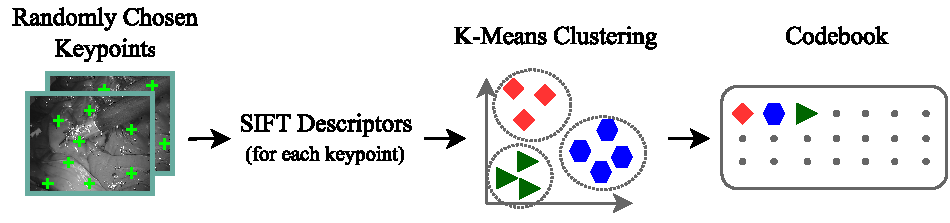
\includegraphics[width=10cm]{bovw/bow_approach_training}
  }
  \\
  \subfloat[BoVW feature encoding phase]
  {
    \label{fig:subfig:bow_coding}
    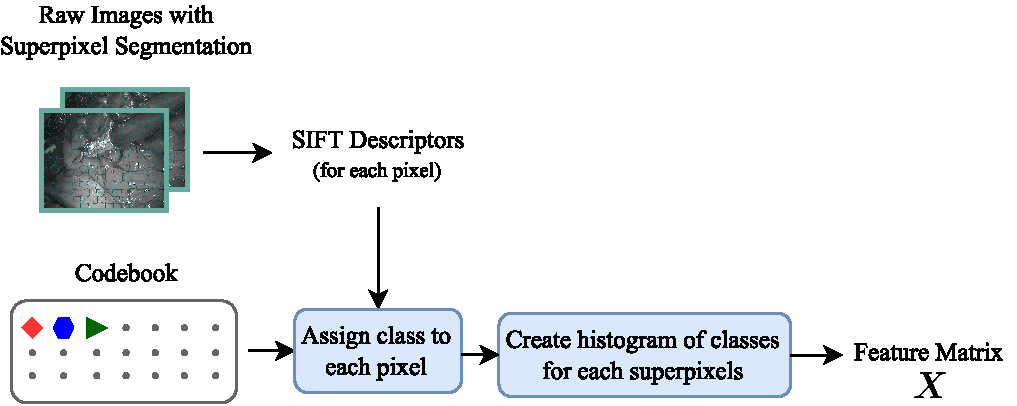
\includegraphics[width=11cm]{bovw/bow_approach_coding}
  }
  \caption[BoVW illustration]{Illustration of \textit{BoVW} approach, divided in two phases. (a) shows the feature learning phase, where SIFT descriptors of randomly chosen keypoints are quantized into a codebook. In the encoding phase (b), each pixel is described by a SIFT descriptor and assigned to a class using the codebook. Subsequently, for each superpixel, a histogram of all assigned classes is created, which makes up the final feature descriptor.}
  \label{fig:BoVW_approch}  
\end{figure}

\subsection{Sparse Coded Spatial Pyramid} \label{scp}
\begingroup
\setlength\intextsep{0pt}
\begin{wrapfigure}[4]{l}[0pt]{1.4cm}
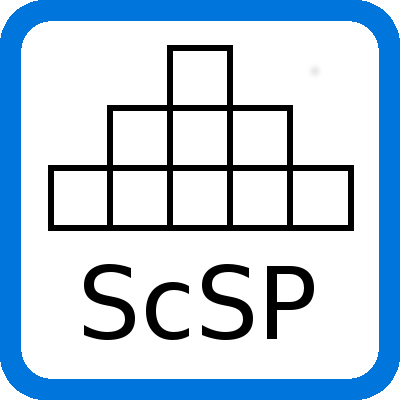
\includegraphics[height=1.5cm]{icons/scsp.png}
\end{wrapfigure}

Another baseline approach, called Sparse-coded Spatial Pyramid (\textit{ScSP}), can be seen as an improved version of the \textit{BoVW} approach with two main modifications. Firstly, instead of using standard k-means clustering, it uses sparse codes of SIFT features, and secondly, a pyramid representation is used. The following describes the added value of \textit{ScSP} with \textit{BoVW}.

\endgroup

%Max pooling instead of standard mean-statistics is not treated [well you just did it... cut and paste that somewhere relevant].

Mathematically, the objective of sparse coding for vector quantization can be written using matrix computation as shown in Eq. \ref{eq:sparse_codes}. The formulations below are adapted from Yang et al. \cite{yang09}.

\begin{samepage}
\begin{equation}
  \min_{\boldsymbol{U,C}} \sum_{m=1}^M \|\boldsymbol{f}_m - \boldsymbol{u}_m \boldsymbol{C}\|^2 + \lambda |\boldsymbol{u}_m|
  \label{eq:sparse_codes} 
\end{equation}
\begin{align*}
  \textrm{subject to } \|\boldsymbol{c}_k\| \leq 1, \hspace{6pt} \forall{k} = 1,2,...,K
\end{align*}
\end{samepage}

Similar to Eq. \ref{eq:k_means}, $\boldsymbol{f_m}$ represents the SIFT appearance vector of keypoint $m$ and $\boldsymbol{C}$ represents the codebook. $\boldsymbol{U} = [\boldsymbol{u}_1,...,\boldsymbol{u}_M]^T \in \mathbb{R}^{M \times K}$ defines the cluster membership indicator. The L2-norm on $\boldsymbol{c}_k$ is typically applied to avoid trivial solutions. If we drop the regularization term $\lambda |\boldsymbol{u}_m|$ and add a cardinality constraint to $\boldsymbol{u}_m$, meaning that only one element in $\boldsymbol{u}_m$ must be nonzero and positive, the sparse coding formulation in Eq. \ref{eq:sparse_codes} simplifies to k-means objective. Yang et al. \cite{yang09} approved that, compared to standard k-means coding, sparse coding can achieve a much lower reconstruction error due to less restrictive constraints. Sparsity also allows the representation to be specialized and capture salient properties of the image.

Lazebnik et al. \cite{lazebnik09} describe the spatial pyramid as a "collection of orderless feature histograms computed over cells defined by a multi-level recursive image decomposition". Fig. \ref{fig:pyramid_repr} show histograms extracted at different locations on an image. The final histogram representation is a concatenation of all histograms from all regions. After normalization, the concatenated histograms can again be seen as a histogram representing the full feature vector. Hence, for the example shown in Fig. \ref{fig:pyramid_repr} using pyramid levels $\boldsymbol{l} = [1,2,4]$, we have a feature dimension $D = K \cdot (1^2 + 2^2 + 4^2) = K \cdot 21$, where $K$ is the number of classes.

\begin{figure}[htbp]
  \centering
  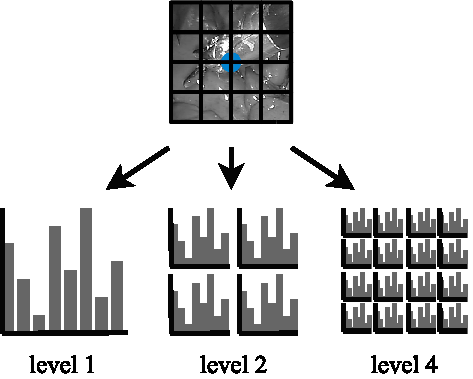
\includegraphics[width=6cm]{scp/pyramid_representation}
  \caption[Spatial pyramid representation]{Illustration of the spatial pyramid representation. Histograms are computed at different levels which are then concatenated into one big vector. After normalization, this vector can again be seen as a histogram vector.}
  \label{fig:pyramid_repr}
\end{figure}

Using a pyramid representation implies that the image patch needs to be square. Intuitively, one wants to enclose within the patch some visual context around the superpixel region. We refer to this parameter as patch size.
In practice, we train our codebook in a similar fashion to \textit{BoVW}, i.e. convert images to grayscale and randomly sample keypoints on every image of the sequence. Each keypoint then gives a SIFT feature vector. Once trained, we extract squared patches of dimension centered on each superpixel's centroid location. We used the implementation of \cite{imdescrip}.

\subsection{Pre-trained VGG-16} \label{vgg}
\begingroup
\setlength\intextsep{0pt}
\begin{wrapfigure}[4]{l}[0pt]{1.4cm}

\includegraphics[height=1.5cm]{icons/vgg.png}
\end{wrapfigure}

VGG is a CNN for large-scale image recognition proposed by \cite{simonyan15}.
The latter work addressed the ImageNet \cite{ILSVRC15} Challenge 2014 (ILSVRC-2014) where it got the first and second places in the localization and classification task, respectively.
Leveraging pre-trained deep networks to address a different task, an approach called transfer learning, has shown its relevance in the frame of semantic segmentation \cite{long15}, emotion recognition \cite{ng15}, and classification \cite{huynh16}.

\endgroup

Here, we use the VGG16 model of \cite{simonyan16}, also known as configuration D \cite[Tab. 1]{simonyan15}.
The model is composed of 16 convolutional layers, each with kernels of size $3 \times 3$.
It is trained for the classification challenge (ImageNet Large Scale Visual Recognition Challenge \cite{ILSVRC15}.
Similar to the \textit{ScSP} approach, we extracted patches at superpixel centroids and fed it to the network.
Since the input dimension of the network is fixed ($244 \times 244 \times 3$), our input data needed to be scaled to that size.
The features are then extracted from the penultimate fully-connected layer, resulting in a feature dimension of $D=4096$.

From a theoretical point of view, let us mention that most machine learning methods make the assumption that training and unseen data lie in the same feature space and have a similar distribution.
However, in many real-world applications, this assumption may not hold \cite{pan2010}.
In a setup where the data distribution of the original training set largely differs from the one we consider, we talk about "Transfer Learning".
We assume that a network pre-trained on a very large-scale dataset with high generalization will produce good features for our task.

\section{Feature Learning: U-Net Based} \label{ch:unet_based}
We now describe our U-Net based feature extraction methods.
We first explain the architecture of the "core" model, i.e. one that will be modified to account for different outputs and loss functions.
We dedicate the second section to data augmentation.
The third section describes how the features can be extracted from the CNN model to obtain feature vectors.
Our various modified U-Nets will then be described in detail.
Finally, an overview summarizes all U-Net based methods.

\subsection{Core Model} \label{model}
Our CNN is a slight modification of the original U-Net structure described in chapter \ref{u_net}. We did not use the U-Net for image segmentation, as initially done by Ronneberger et. al. Instead, we trained the network in an unsupervised manner, like an autoencoder, on our data and extracted features at the lowest level. Some of our methods operate in a weakly-supervised fashion, where information related to the gaze location is used as a prior.

Fig. \ref{fig:unet_model} shows a modified U-Net structure. Similar to the original structure, we used two stacked convolution layers with $3 \times 3$ filter size and stride $1$ per level. Since we want the output to be the same size as the input, we used zero padding instead of valid padding. Thus, we modified the structure by adding a batch normalization layer with ReLU activation after the convolutional layers. Configurations of max-pooling did not change. Instead of using up-convolutional layers in the expansive path, we used upsampling layers, which apply a simple nearest neighbor interpolation to increase the resolution.

As shown in \cite{vorontsov17}, this last modification improves prediction performances.  In addition, upsampling layers are parameter-free and allow to reduce the memory requirement. The very last layer is a convolutional layer with filter size $1 \times 1$ and sigmoid activation. That our output value is between $0$ and $1$ is assured by the use of a last sigmoid activation layer.

In contrast with our baseline approaches, our U-Net methods take as input the full image instead of patches.
How the features are then assigned to the individual superpixel is described in chapter \ref{feat_extract}.
Max pooling downscales the resolution by $2$. Thus, the lowest resolution at the deepest layer is given by the input resolution divided by $2^4=16$. This implies that input image resolution must be dividable by 16. Hence, input images were downscaled to the nearest width and height which are dividable by $16$ before fed to the network. The number of input, as well as output channels, differ between the individual U-Net methods. In what follows, we refer to $c\_i$ as the number of input channels and $c\_o$ as the number of output channels. We normalized the inputs to have zero mean and a variance of $1$.

The use of batch normalization layers helps for optimization, as shown in chapter \ref{optimization}.
Since GPU memory is limited and data input resolution is rather large, we are restricted to small mini-batch sizes.
According to Gastaldi et al. \cite{gastaldi17}, batch normalization also has a regularization effect due to fluctuations in mini-batch statistics. Especially with small mini-batches, those fluctuations regularize the network.

\clearpage
\begin{figure}[!htbp]
  \centering
  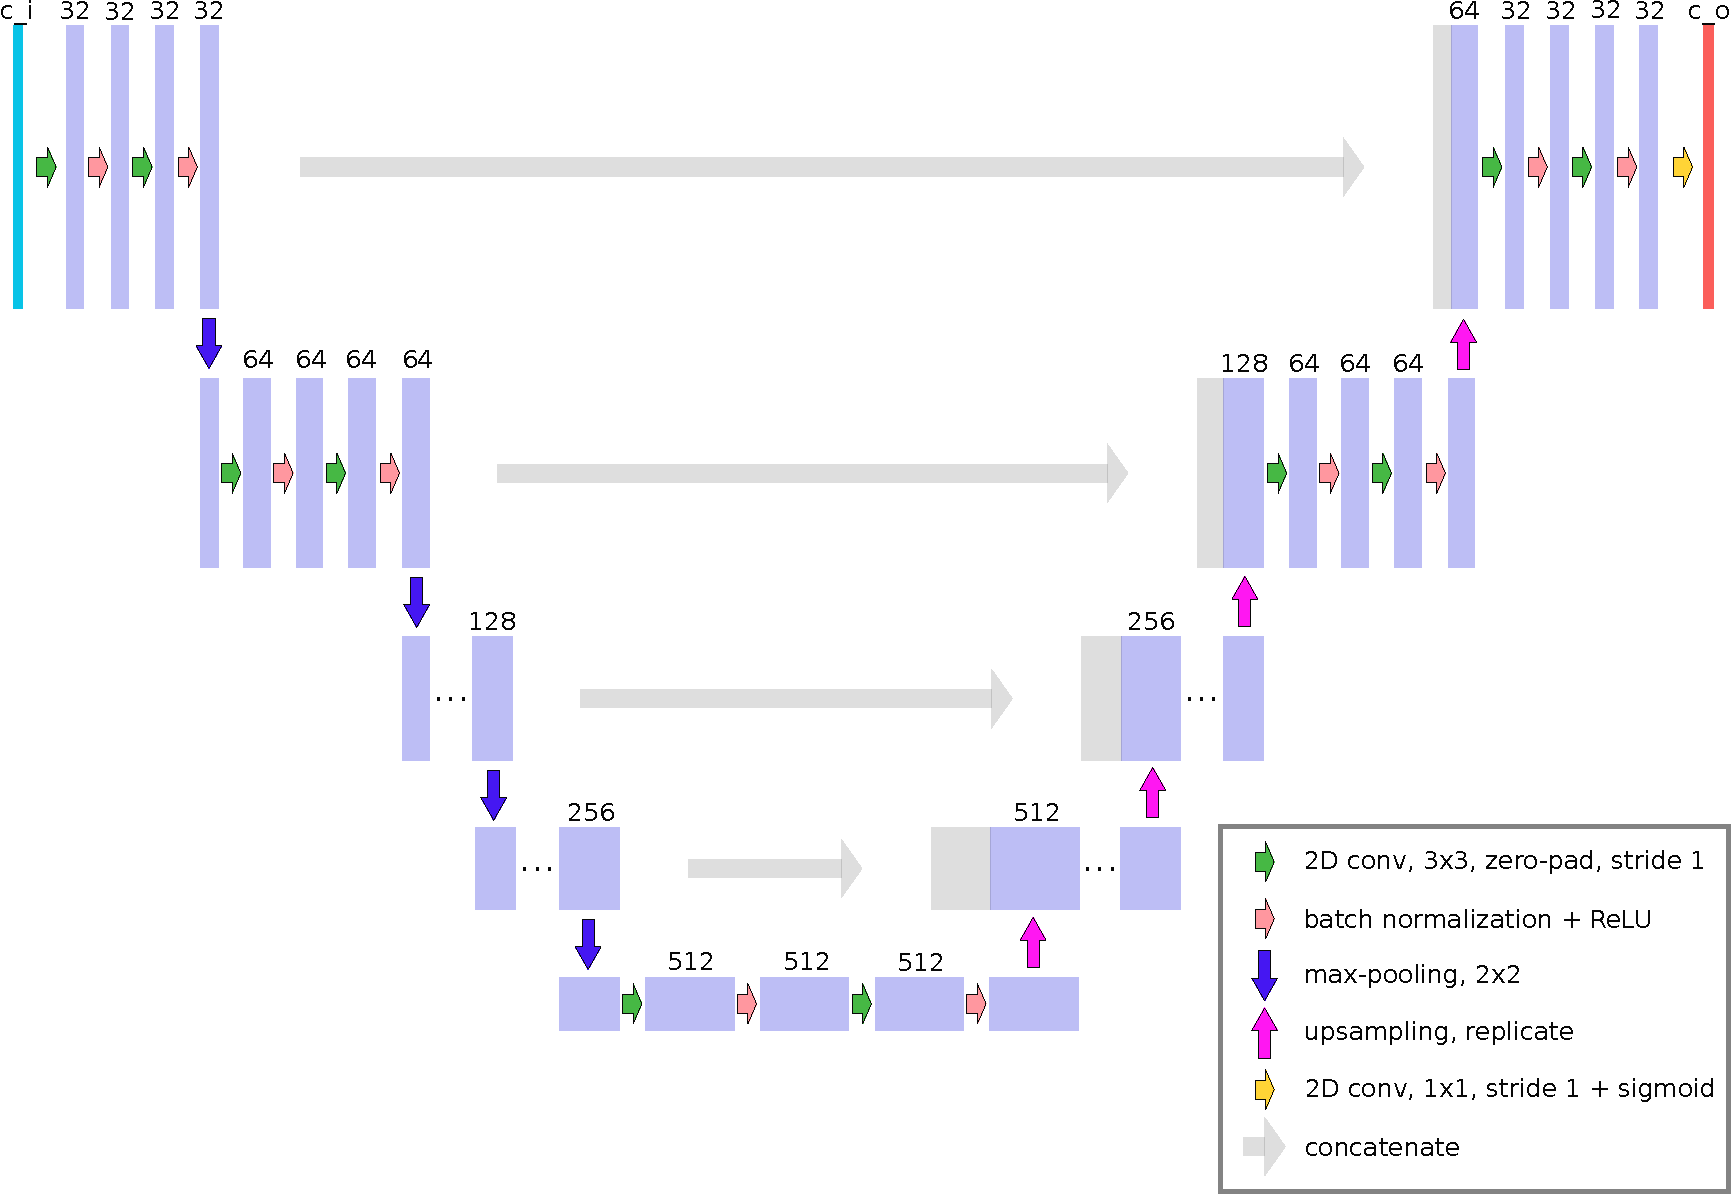
\includegraphics[width=\textwidth]{unet/model5}
  \caption[Modified U-Net architecture]{Illustration of our modified U-Net structure. Other than the original U-Net structure, it has a batch normalization layer after each convolutional layer. Depending on the data color space and loss function, it uses different number of input channels $c\_i$ and output channels $c\_o$.}
  \label{fig:unet_model}
\end{figure}

\subsection{Data Augmentation} \label{ch:data_gen}
Since the datasets we used are rather small in size, we used data augmentation wherever possible to increase the training data size. However, since we have a setting where we train the neural network on the same data we later extract the features from, the model does not need to generalize to non-seen data. Hence, we only use image transforms that are observed within the data. For example, it is very likely that during a slit-lamp recording the user rotates and shifts the camera, resulting in different angles and positions of the optical disc. This confirms to use horizontal and vertical shift, as well as rotation for image transforms. Contrarily, as the size of the object seldom changes, scaling and zooming are not relevant transformations.
The same reasoning applies to other datasets.
To sum up, we resort to rotation, vertical/horizontal translation as well as little shearing. Additionally, we added Gaussian noise for regularization. In our implementation, we used the online data generator provided by the Keras framework \cite{Keras}, which randomly generates new data during training time. Some examples and parameters used are described in chapter \ref{results_data_gen}.

\clearpage
\subsection{Feature Extraction} \label{feat_extract}
Similarly to our baseline methods, U-Net based methods construct a feature matrix $\boldsymbol{X} = [\boldsymbol{x}_1,...,\boldsymbol{x}_S]^T \in \mathbb{R}^{S \times D}$ describing each superpixel. Fig. \ref{fig:feat_extract} illustrates this process on an example of a single image. After training, a forward pass is performed on all image and features are taken as the output (ReLU) of the deepest layer. Those features correspond to a downscaled version of the input image. Hence, it must be upscaled to the original image resolution. Each feature dimension is independently upscaled to the original image size using bicubic interpolation. Since one pixel becomes a region, extrapolation is also needed at border regions, shown by the red circle and square in Fig. \ref{fig:feat_extract}. As we now have a descriptor for each pixel upscaled to the same resolution as the original data, we can take the mean over all descriptors belonging to the individual superpixels with feature dimension $D=512$.
\vspace{10pt}

\begin{figure}[htbp]
  \centering
  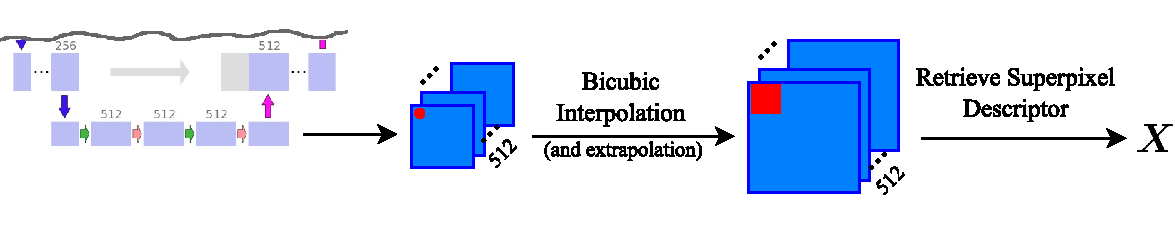
\includegraphics[width=\textwidth]{feat_extract/feature_extraction}
  \caption[Feature extraction model]{Illustration of feature extraction for U-Net based methods. The features are extracted from the deepest level. Those features are then interpolated (and extrapolated) on each dimension individually to obtain the original resolution. Each pixel is described by a feature vector of dimension $D=512$.
    Superpixels are assigned to the mean of all feature vectors that it envelopes.}
  \label{fig:feat_extract}
\end{figure}

\subsection{U-Net Reconstruct}
\begingroup
\setlength\intextsep{0pt}
\begin{wrapfigure}[4]{l}[0pt]{1.4cm}
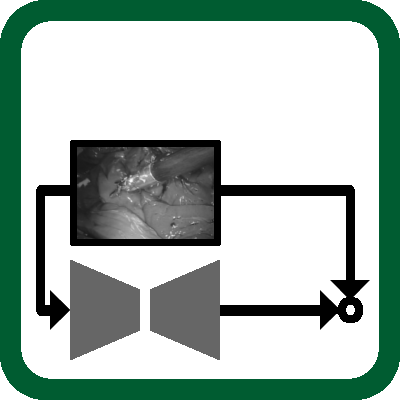
\includegraphics[height=1.5cm]{icons/unet_rec.png}
\end{wrapfigure}

\textit{U-Net Reconstruct} (or \textit{U-Net Rec}) is an unsupervised model. It takes as input the image data and reconstructs the same data. Let $\mathcal{I}$ be the image set and $\boldsymbol{I}_k \in [0,1]^{H \times W \times C}$ an image with height $H$, width $W$ and number of channels $C$. We assume that $\boldsymbol{I}_k$ is already downscaled to have $H$ and $W$ dividable by $16$ (see chapter \ref{model}). Pixels are described by $\boldsymbol{I}_k(i,j,c) \in [0,1]$ with $i$ and $j$ its indices. The reconstructed image, of same dimension as the input, is written $\boldsymbol{\hat{I}}_k$. The network's channel dimensions is taken as $C = c_i = c_o$. We chose to use a mean-squared error (MSE) loss function. For a minibatch of size $B$, the loss is given by:

\endgroup
\vspace{6pt}

\begin{equation}
L_{MSE} = \frac{1}{W H |\mathcal{B}|} \sum_{\boldsymbol{I}_l \in \mathcal{B}} \sum_{i,j,c} \|\boldsymbol{I}_l(i,j,c) - \boldsymbol{\hat{I}}_l(i,j,c)\|^2
\label{eq:mse_loss}
\end{equation}
\vspace{6pt}

Where $\| \cdot \|$ is the $L2$-norm and $\mathcal{B} \subset \mathcal{I}$ is the minibatch.
In later formulations, we will omit the summation on the mini-batch for clarity.

\clearpage
\subsection{U-Net Gaze Reconstruct} \label{unet_gaze_rec}
\begingroup
\setlength\intextsep{0pt}
\begin{wrapfigure}[4]{l}[0pt]{1.4cm}
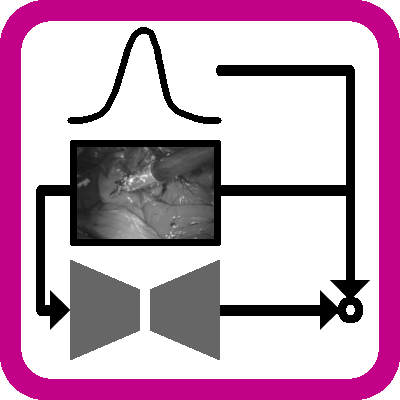
\includegraphics[height=1.5cm]{icons/unet_gaze_rec.png}
\end{wrapfigure}

Similar to \textit{U-Net Rec}, \textit{U-Net Gaze Reconstruct} (or \textit{U-Net Gaze Rec}) trains the network in an autoencoder fashion. This time, we introduce a prior on the gaze location into the loss-function. Let $\boldsymbol{g} = [g_x, g_y]$ be the xy-coordinates of the gaze-point, and  $\boldsymbol{Z} \in [0,1]^{H \times W}$ a probability map. Assuming that the gaze location $\boldsymbol{g}$ is given for an image $\boldsymbol{I}$, we take $\boldsymbol{Z} \sim \mathcal{N}(\boldsymbol{g}, \sigma^2\mathbb{I})$, a 2D-Gaussian distribution with standard deviation $\sigma$ and mean $\boldsymbol{g}$. For images where no gaze locations are available, we take a Uniform distribution. It is formulated in Eq. \ref{eq:gaussian}.

\endgroup

\begin{equation}
\boldsymbol{Z} = 
\begin{cases}
  \mathcal{U}(0,WH),& \textit{if } \boldsymbol{g} \textit{ not available}\\         \mathcal{G}(\boldsymbol{g}, \sigma^2\mathbb{I}),         & \textit{if } \boldsymbol{g} \textit{ available}
\end{cases}
\label{eq:gaussian}
\end{equation}
\hspace{6pt}

$\boldsymbol{Z}_{i,j}$ therefore models the object prior at location $(i,j)$, with $i \in \{\mathbb{Z} \mid 1 \leq i \leq H\}$ and $j \in \{\mathbb{Z} \mid 1 \leq j \leq W\}$ to be the probability of that pixel corresponding to the object of interest. Each pixel's $L2$-norm is then multiplied by $\boldsymbol{Z}_{i,j}$. The loss function is therefore given by:

\begin{equation}
L_{MSE\_Gaze} = \frac{1}{W H} \sum_{i,j} \frac{\boldsymbol{Z}_{i,j}}{\max{\{\boldsymbol{Z}\}}} \|\boldsymbol{I}_{i,j} - \boldsymbol{\hat{I}}_{i,j}\|^2
\label{eq:mse_gaze_loss}
\end{equation}
\hspace{6pt}

Where we normalize by $\max{\{\boldsymbol{Z}\}}$ for later comparison with the loss of \textit{U-Net Rec}. This model, therefore, penalizes errors situated near the gaze-point. In most image modalities, the object of interest is only a small portion of the image and distinctive. Contrarily, the background is rather regular or even fully black, as it usually is for CT and MRI scans. Hence, we can reason that penalizing the loss in regions of interest equalizes the weights given to background and object of interest in terms of area occupied by the foreground, resp. background.

\subsection{U-Net Gaze Probability Map} \label{unet_gaze_prob_map}
\begingroup
\setlength\intextsep{0pt}
\begin{wrapfigure}[4]{l}[0pt]{1.4cm}
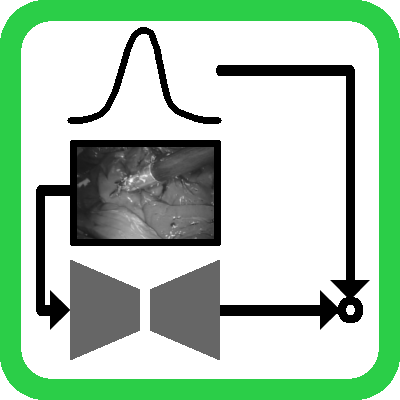
\includegraphics[height=1.5cm]{icons/unet_gaze_prob.png}
\end{wrapfigure}

\textit{U-Net Gaze Probability Map} (or \textit{U-Net Gaze Prob}) predicts a probability map of the gaze location given the image. We use the same formulation for the probability map $\boldsymbol{Z}$ as for \textit{U-Net Gaze Rec} method in chapter \ref{unet_gaze_rec}. The model's output is now given by $\boldsymbol{\hat{Z}} \in [0,1]^{H \times W}$. In the work of Kurmann at al. \cite{kurmann17}, they used a similar setting and showed that a binary-cross-entropy loss (BCE-loss) performs well. This gave rise to use BCE-loss, formulated in Eq. \ref{eq:mse_gaze_prob_loss} on an example of one image. The network's channel dimensions are $c\_i=C$ and $c\_o=1$.

\endgroup
\begin{equation}
L_{BCE} = \frac{1}{W H} \sum_{i,j} \boldsymbol{Z}_{i,j} \log{\boldsymbol{\hat{Z}}_{i,j}} + (1-\boldsymbol{Z}_{i,j}) \log{(1-\boldsymbol{\hat{Z}}_{i,j})}
\label{eq:mse_gaze_prob_loss}
\end{equation}
\hspace{6pt}

\clearpage
\subsection{U-Net Gaze Probability Map Freezed}
\begingroup
\setlength\intextsep{0pt}
\begin{wrapfigure}[4]{l}[0pt]{1.4cm}
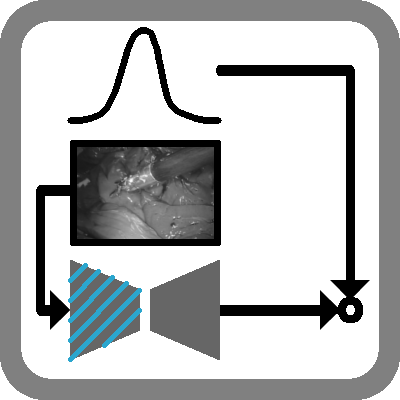
\includegraphics[height=1.5cm]{icons/unet_gaze_prob_freeze.png}
\end{wrapfigure}

\textit{U-Net Gaze Probability Map Freezed} (or \textit{U-Net Gaze Prob Freeze}) combines the benefits of \textit{U-Net Rec} and \textit{U-Net Gaze Prob}. The model is first trained as an autoencoder similarly to \textit{U-Net Rec}. Encoder weights are then frozen (or fixed), and the model is re-trained in a similar fashion to \textit{U-Net Gaze Prob}. Fig. \ref{fig:model_freeze} shows the network's portion where weights are frozen. We can see that the only layers that affect the feature extraction are the ones located at the lowest level. This method is aimed at leveraging benefits of an autoencoder setting in \textit{U-Net Rec} and benefits by using the gaze prior as in \textit{U-Net Gaze Prob}.

\endgroup

\begin{figure}[htbp]
  \centering
  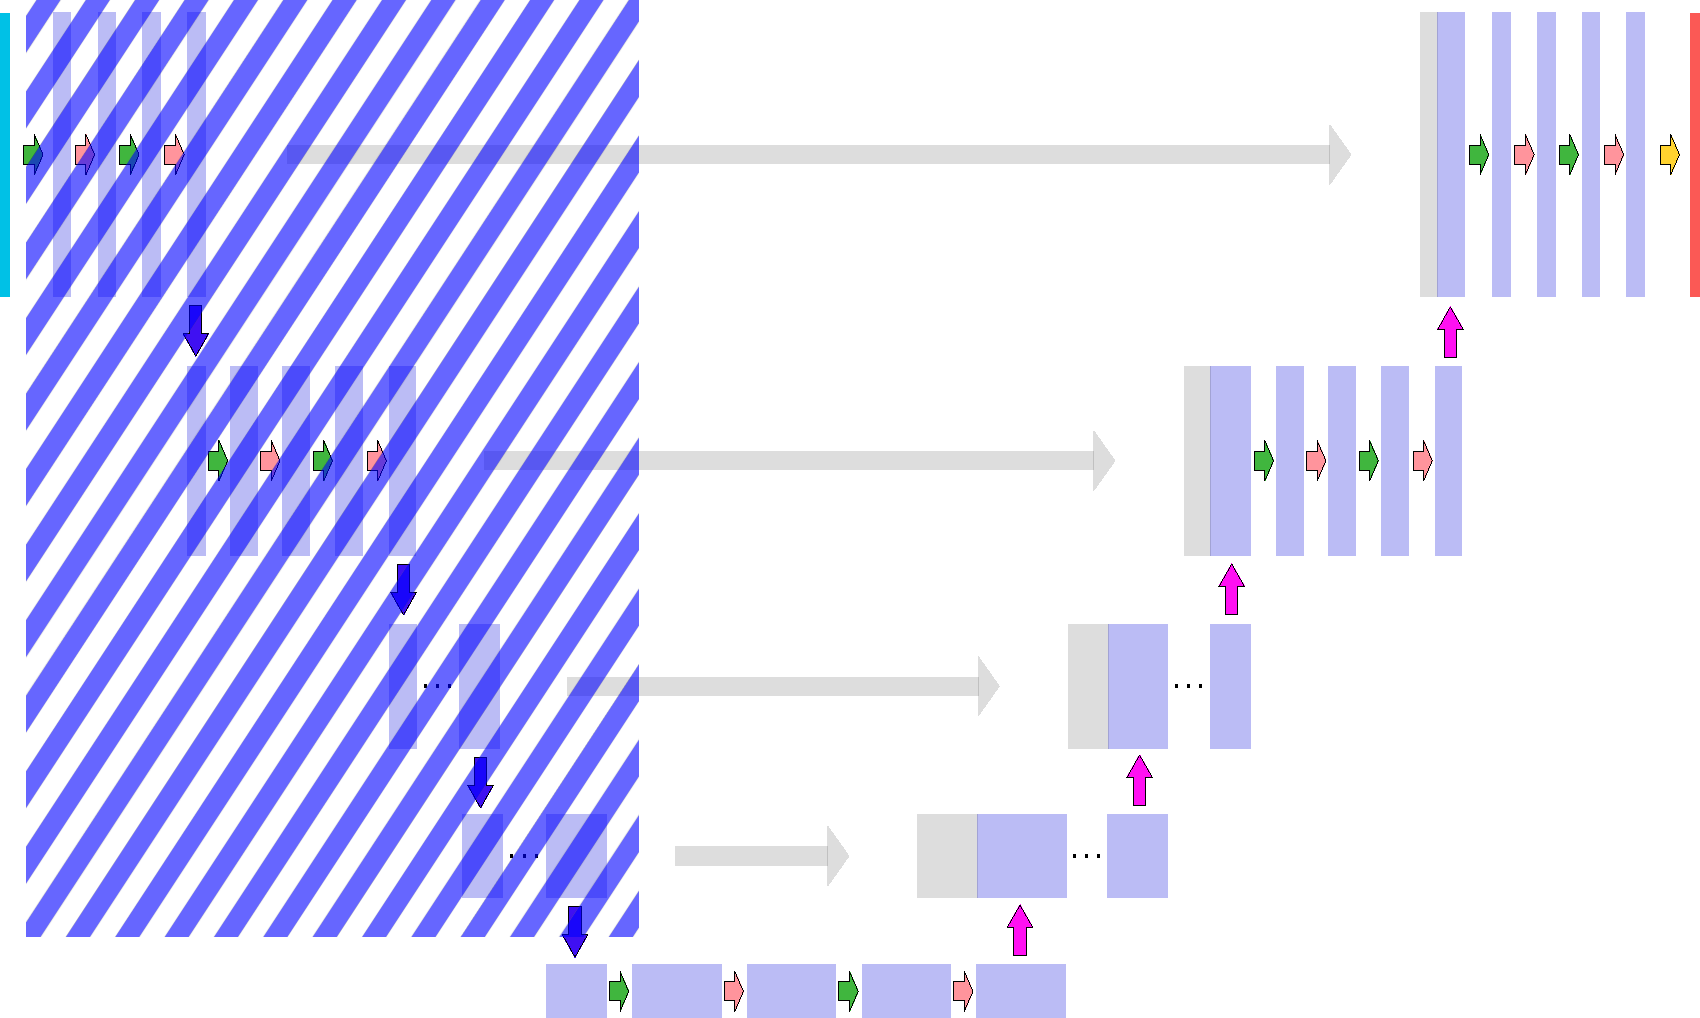
\includegraphics[width=5.0cm]{unet/model5_coarse}
  \caption[Modified U-Net with freezed encoder part]{Illustration of frozen layers in \textit{U-Net Gaze Prob Freeze} method. All encoder part except the lowest level is frozen.}
  \label{fig:model_freeze}
\end{figure}

\subsection{U-Net Gaze Probability Map Concatenate} \label{unet_gaze_prob_concat}
\begingroup
\setlength\intextsep{0pt}
\begin{wrapfigure}[4]{l}[0pt]{1.4cm}
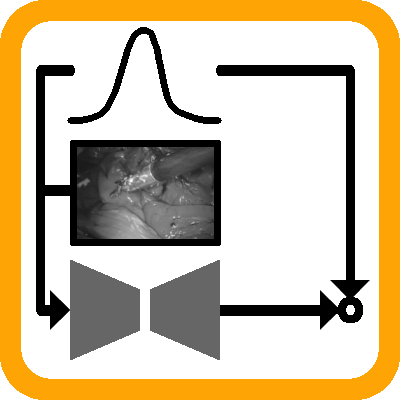
\includegraphics[height=1.5cm]{icons/unet_gaze_prob_concat.png}
\end{wrapfigure}

This model is based on the assumption that objects of interest in our context have relatively slow motion. In other words, the current gaze location is correlated to the previous gaze location(s). We therefore aim at predicting the object's current location. \textit{U-Net Gaze Probability Map Concatenate} (or \textit{U-Net Gaze Prob Concat}) incorporates the data's temporal correlation.

\endgroup

Similar to \cite{lea16}, who investigated the problem of fine-grained action segmentation, we increased the model's number of input channel by a motion image. However, we followed a more straightforward approach by adding as motion information the previous probability map $\boldsymbol{Z}^{(t-1)}$.

Fig. \ref{fig:unet_gaze_concat} illustrates the overall structure on one image $\boldsymbol{I}$. The gaze probability map at time $t-1$, shown as $\boldsymbol{Z}^{(t-1)}$, is concatenated to $\boldsymbol{I}^{(t)}$. These taken as inputs are then used to predict the gaze location at time $t$, defined by $\boldsymbol{\hat{Z}}^{(t)}$. Similar to \textit{U-Net Gaze Prob}, we used BCE-loss.

\begin{figure}[htbp]
  \centering
  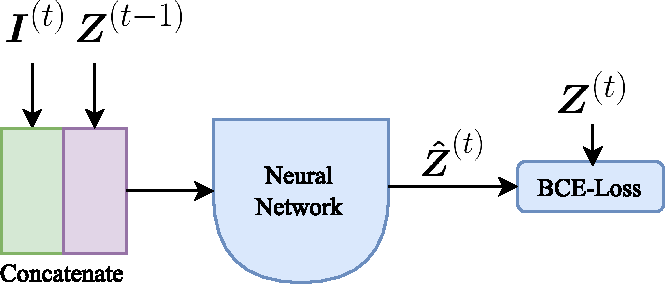
\includegraphics[width=7cm]{unet/unet_gaze_concat}
  \caption[Structure of U-Net Gaze Prob Concat]{Structure of U-Net based method \textit{U-Net Gaze Prob Concat}. The previous gaze probability map $\boldsymbol{Z}^{(t-1)}$ is concatenated to the current image data $\boldsymbol{I}^{(t)}$. Out of those informations, the Neural Network predicts the current gaze location $\boldsymbol{Z}^{(t)}$.}
  \label{fig:unet_gaze_concat}
\end{figure}

Since we augmented the inputs by an additional channel, the model's channel dimension become $c\_i=C+1$ and $c\_o=1$. Note that in this configuration, the ordering of input frame is substantial. Thus, it made it difficult to apply data augmentation procedure. Due to time limitations, we did not use data augmentation.

\subsection{U-Net Gaze Probability Map LSTM} \label{ch:unet_gaze_prob_lstm}
\begingroup
\setlength\intextsep{0pt}
\begin{wrapfigure}[4]{l}[0pt]{1.4cm}
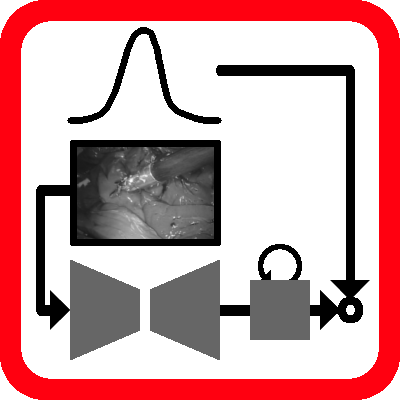
\includegraphics[height=1.5cm]{icons/unet_gaze_prob_lstm}
\end{wrapfigure}

\textit{U-Net Gaze Probability Map LSTM} (or \textit{U-Net Gaze Prob LSTM}) also incorporates the temporal correlation of the object. It uses three models from \textit{U-Net Gaze Prob} with shared weights to predict three consecutive gaze probability maps. Those predicted probability maps are again fed to a recurrent unit, more precisely a convolutional long-short-term-memory (CLSTM) \cite{shi15}, to predict the next gaze location. Fig. \ref{fig:unet_gaze_lstm} illustrates this structure. The CLSTM uses filters of size $3 \times 3$ and no return sequence.

\endgroup

\begin{figure}[htbp]
  \centering
  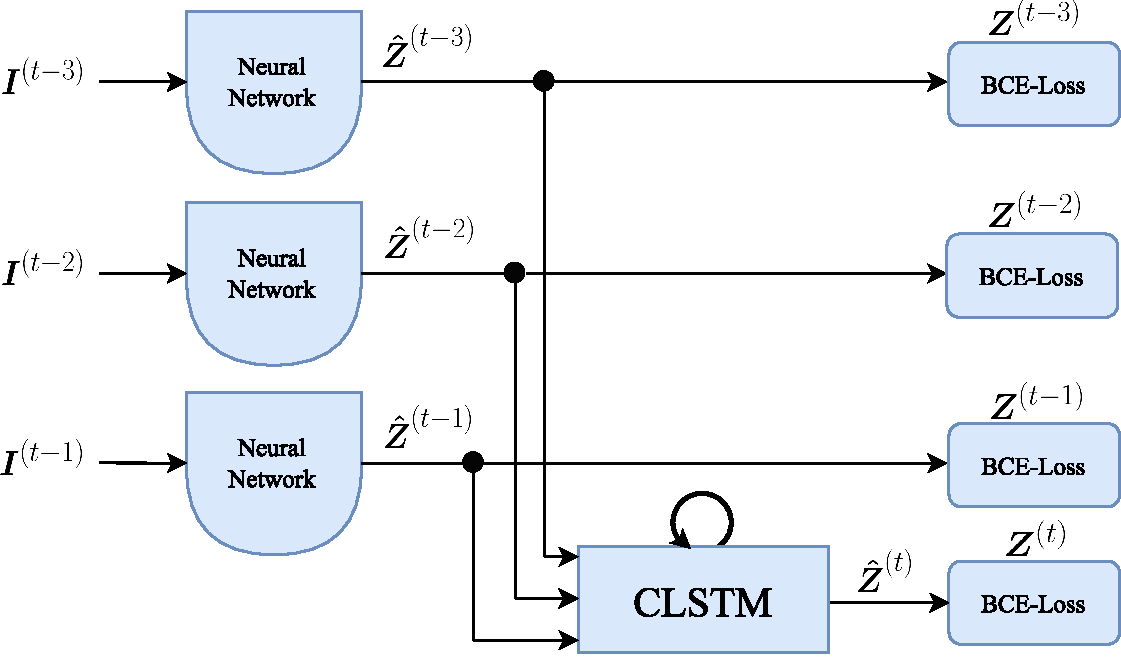
\includegraphics[width=10cm]{unet/unet_gaze_lstm}
  \caption[Structure of U-Net Gaze Prob Map LSTM]{Structure of U-Net based method \textit{U-Net Gaze Prob LSTM}. A sequence of three images is fed to three identical U-Net models as in \textit{U-Net Gaze Prob} with shared weights. The predicted gaze probability maps $\boldsymbol{\hat{Z}}$ are fed to a CLSTM, predicting the next gaze. The overall loss is a mix of all four BCE-losses.}
  \label{fig:unet_gaze_lstm}
\end{figure}

The overall loss $L_{BCE\_LSTM}$ for one image sequence of three images is shown in Eq. \ref{eq:bce_lstm}. $L_{BCE}(A,B)$ defines the binary cross entropy, formulated in Eq. \ref{eq:mse_gaze_prob_loss}, between $A$ and $B$. Parameter $\alpha$ is used to adjust the weight of the CLSTM prediction. We used some jittering to represent the data, i.e. one sample is given by the sequence $[\boldsymbol{I}^{(t=0)}, \boldsymbol{I}^{(t=1)}, \boldsymbol{I}^{(t=2)}]$, and $[\boldsymbol{I}^{(t=1)}, \boldsymbol{I}^{(t=2)}, \boldsymbol{I}^{(t=3)}]$ represents another sample. Likewise to the method \textit{U-Net Gaze Prob Concat}, we did not synthesize more data by using any sort of data augmentation.

\begin{equation}
L_{BCE\_LSTM} = \alpha \Big[\sum_{d=1}^3 L_{BCE}(\boldsymbol{\hat{Z}}^{(t-d)}, \boldsymbol{Z}^{(t-d)})\Big] + (\alpha - 1) L_{BCE}(\boldsymbol{\hat{Z}}^{(t)}, \boldsymbol{Z}^{(t)})
\label{eq:bce_lstm}
\end{equation}
\hspace{6pt}

\clearpage
\subsection{U-Net Based Methods Overview}
Tab. \ref{tab:summary_unet_methods} summarizes the U-Net based methods. To recap, $C$ is the number of image channels ($1$ for grayscale and $3$ for colored) and $c\_i$, $c\_o$ the number of the networks input and output channels, respectively.

\begin{table}[!htbp]
   \centering
   \caption[U-Net based method overview]{Overview of U-Net based methods with $C$ being the number of channels in the images and $c\_i$, $c\_o$ the network's input and output channel dimension, respectively.}
   \begin{tabular}{l|m{1.3cm}|c|c|c|c}
      \toprule
      \textbf{Method} & \textbf{Symbol} & \textbf{Inputs} & \textbf{Labels} & \textbf{c\_i} & \textbf{c\_o} \\
      \midrule
      U-Net Rec & 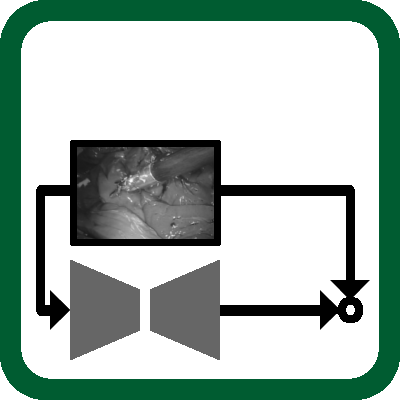
\includegraphics[width=1cm]{icons/unet_rec.png} & Image & Image & $C$ & $C$ \\
      \midrule
      U-Net Gaze Rec & 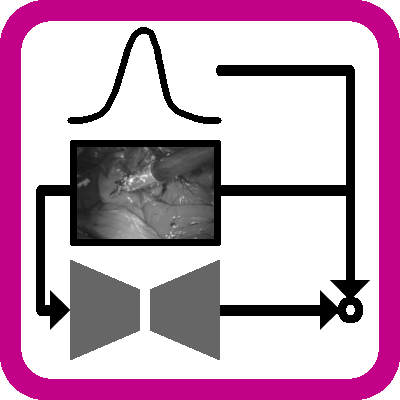
\includegraphics[width=1cm]{icons/unet_gaze_rec.png} & Image & Image \& Gaze & $C$ & $C$ \\
      \midrule
      U-Net Gaze Prob & 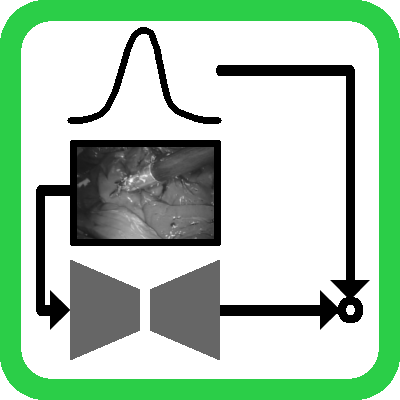
\includegraphics[width=1cm]{icons/unet_gaze_prob.png} & Image & Gaze & $C$ & $1$ \\
      \midrule
      U-Net Gaze Prob Freeze & 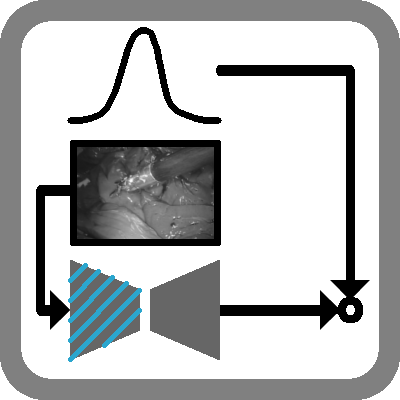
\includegraphics[width=1cm]{icons/unet_gaze_prob_freeze.png} & Image & Gaze & $C$ & $1$ \\
      \midrule
      U-Net Gaze Prob Concat & 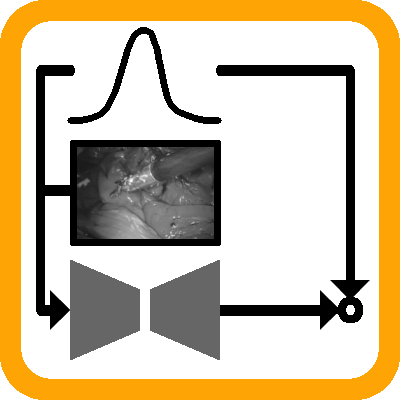
\includegraphics[width=1cm]{icons/unet_gaze_prob_concat.png} & Image \& Gaze & Gaze & $C+1$ & $1$ \\
       \midrule
      U-Net Gaze Prob LSTM & 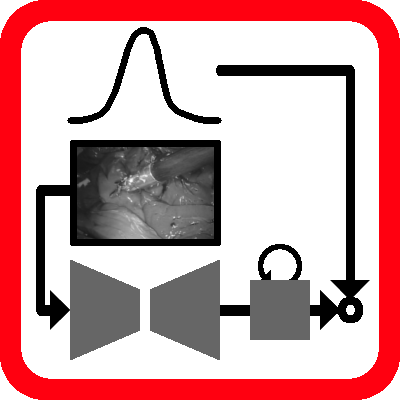
\includegraphics[width=1cm]{icons/unet_gaze_prob_lstm.png} & Image Sequence & Gaze & $3 \times C$ & $3 \times 1$ \\
      \bottomrule
   \end{tabular}
   \label{tab:summary_unet_methods}
\end{table}

%\myworries{
%\begin{itemize}
%  \item Training time (one paragraph)
%\end{itemize}}

\section{Evaluation Method}
We used a random forest classifier to compare the performance between the different feature learning methods. How this classifier is applied and configured, is described in a first section. Later, we describe the measures, which allow us to compare the performance among one another method.

\subsection{Random Forest} \label{random_forest}
To compare performance between the elaborated methods, we set up a Random Forest classifier, as shown in Fig. \ref{fig:random_forest}.
It takes as input a feature matrix $\boldsymbol{X} \in \mathbb{R}^{S \times D}$ and labels $\boldsymbol{y} \in \{0,1\}^{S}$ of one image data sequence.
As described in chapter \ref{framework}, $S$ is the number of superpixels in one sequence and $D$ the feature dimension.
Firstly, labels $\boldsymbol{y}$ and feature matrix $\boldsymbol{X}$ are both similarly shuffled.
Then, it uses k-fold cross-validation on $5$ folds to train the classifier and validate.
This ensures that each data point belonged one time to the validation set $\boldsymbol{X}_V$, resp. $\boldsymbol{y}_V$ and $4$ times to the training set $\boldsymbol{X}_T$, resp. $\boldsymbol{y}_T$. All $5$ validation sets are individually evaluated, a precision-recall curve drawn as well as a \textit{max F1-Score} calculated. The final performance measure is the average over all $5$ folds. Since we usually have very few positive labels, we paid attention that each validation set contains more or less the same number of positive labels.

\begin{figure}[htbp]
  \centering
  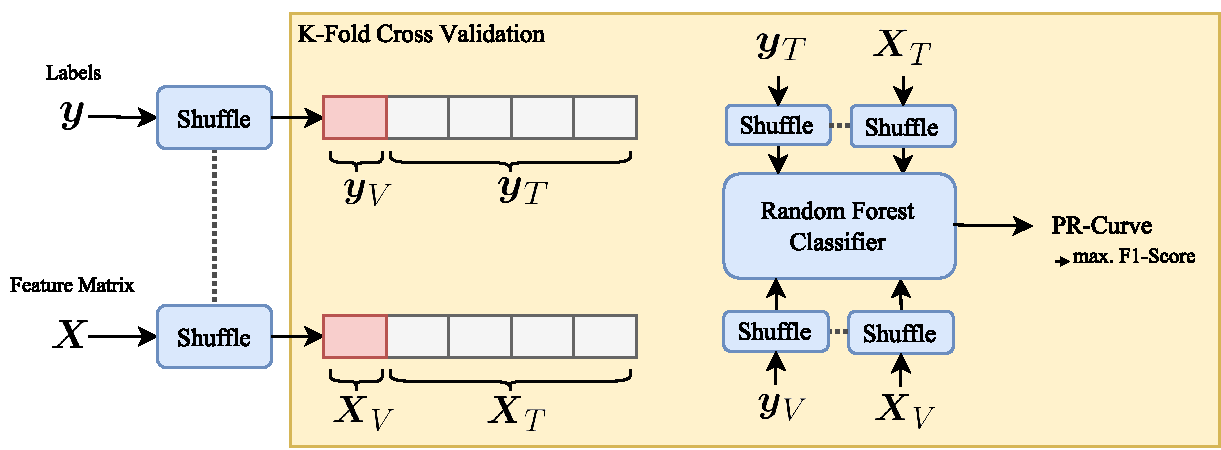
\includegraphics[width=14cm]{random_forest/random_forest}
  \caption[Illustration of Random Forest classifier]{Set-up of Random Forest classifier for evaluating performance of feature learning methods. It learns a Random Forest classifier on superpixel labels $\boldsymbol{y}$ and feature matrix $\boldsymbol{X}$ of one image data sequence. Since the datasets are rather small in size and have few positive labels, validation is done by a k-fold cross-validation.}
  \label{fig:random_forest}
\end{figure}

In our Random Forest classifier, all nodes are expanded until the leaves are pure.
There is a big discussion whether pruning trees help random forest for better performance.
Segal \cite{segal04} revealed that gains can be obtained by regulating tree size.
However, \cite[pg. 596]{hastie09} notices that those performance gains are rather small. We stuck to Hastie et al.'s conclusion and took advantage of one less tuning parameter.

We built the forest out of $150$ trees and used $m=\sqrt{p}$, where $m$ is the number of selected predictor variables and $p$ the number of all predictor variables. For implementation, we used the sklearn package \cite{scikit-learn}.

\subsection{Precision-Recall Curve}
Precision Recall curves (PR-curves) are a performance measure commonly used for binary decision problems in machine learning.
We used PR-curves to evaluate the results of our Random Forest classifier, and thus, PR-curves present the performance of a feature learning method on a dataset.
We also tried using Receiver Operation Characteristics (ROC) as a measure, but it turned out that PR-curves are a more useful measure for our data.
This might be due to the nature of our data.
Since we usually have much more negative than positive labels, our data becomes skewed.
PR-Curves are more informative than ROC for skewed data, as pointed out by \cite{davis06}. They also stated that a curve dominates in ROC space if and only if it dominates in PR space.

As described in chapter \ref{random_forest}, the final performance measure of an algorithm is the average over all five cross validation folds. By this means, the variance is minimized.

\clearpage
\subsection{Max F1-Score} \label{ch:scores}
F1-Score is a measure that considers both, recall and precision. It's best value is reached at $1$ and worst at $0$. The formula is given by Eq. \ref{eq:f1_score}.

\begin{equation}
\textrm{F1-Score} = 2 \cdot \frac{\textrm{Precision} \cdot \textrm{Recall}}{\textrm{Precision} + \textrm{Recall}}
\label{eq:f1_score}
\end{equation}
\hspace{6pt}

\textit{Max F1-Score} is defined as the relationship between precision and recall that reaches the maximum score. It can be seen as calculating for all points in a PR-curve, their according F1-Scores and taking the maximum. An example is given in Fig. \ref{fig:f1_score}, where the left diagram shows a PR-curve and the right diagram the F1-Score given the Recall values. The maximum value is shown in green.

\begin{figure}[ht]
  \centering
  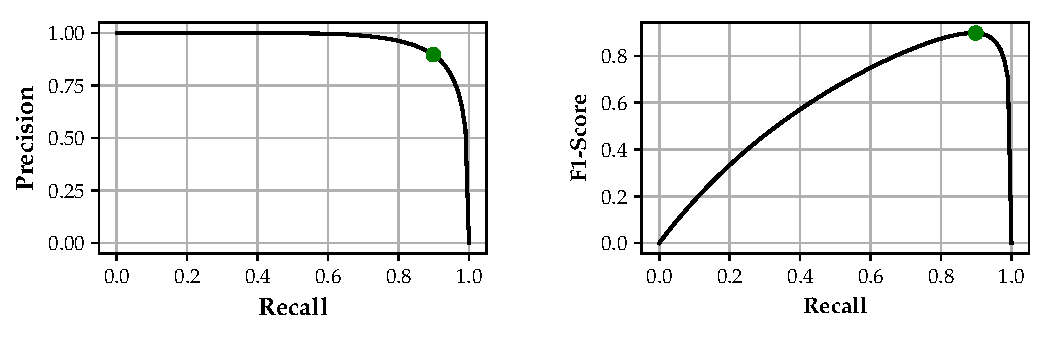
\includegraphics[width=11cm]{f1_score/f1_score}
  \caption[Illustration of max F1-Score]{Illustration of \textit{max F1-Score}. The left diagram shows an example of a \textit{Precision Recall curve}. The diagram on the right shows the F1-Score given the \textit{Recall} values. Maximum score is marked by a green point, the \textit{max F1-Score}.}
  \label{fig:f1_score}
\end{figure}

%%% Local Variables:
%%% mode: latex
%%% TeX-master: "../../main"
%%% End:
